\documentclass{article}
\usepackage{times}
\usepackage{graphicx}
\usepackage{amsmath}
\usepackage{subfigure} 
\usepackage{algorithm}
\usepackage{algorithmic}
\usepackage{hyperref}
\usepackage{float}

\newcommand{\theHalgorithm}{\arabic{algorithm}}

\usepackage[accepted]{icml2015} 

\icmltitlerunning{Final Project Report}
\title{Final Project Report}

\begin{document} 
\twocolumn[
\icmltitle{Final Project Report}
\icmlauthor{Samuel Cuthbertson}{samuel.cuthbertson@colorado.edu}
\icmlauthor{Connor Hudson}{connor.c.hudson@colorado.edu}

\vskip 0.3in
]
\section*{Abstract}
The purpose of this project is to create a method for predicting the best households to advertise to, given a training set of spending amount and anonymized sparse features. To combat the extreme skew of the data, we explore a method of training a classifier to predict zero or non-zero spending using multiple uniformly distributed "zero classes". We use the results from this classifier to rank spending amounts using a linear regression trained on log-transformed non-zero spending data. Our algorithm results in achieving 60\% of possible total revenue, comparable to industry average and significantly better than random guessing, which achieves less than 10\%. 


\section*{Introduction}
For this project, we competed in the Oracle Data Cloud Audience Competition \cite{codata_oracle_2016} as part of the CU Boulder Data Science Team. The competition itself is organized around three large data sets, designated as \texttt{train}, \texttt{val}, and \texttt{contest}. Both \texttt{train} and \texttt{val} are composed with two labels (Household Id and Household Spending) and a sparse feature vector, while \texttt{contest} has only Household Id as a label. The purpose of the competition was to predict whether or not to advertise to a given household. In full, we got to select $100,000$ households from the \texttt{contest} set and would be scored on what percentage of those $100,000$ were spenders, as well as what percentage of total possible revenue we achieved through advertising to those $100,000$ households. It was assumed that advertising to a household would make that household spend, and that not advertising to a household would mean they wouldn't spend. 

For more specifics about the structure of the given data and scoring of the competition, see Appendix \ref{sec:app1}.

\section*{Methods}
Initially, we separated it out into two separate problems: a classification problem of whether or not a household would spend any money, and a regression problem of how much money that household would spend. In fitting with that methodology, this methods section will be likewise split. However, it's worth noting that we exclusively used Vowpal Wabbit \cite{langford_johnlangford/vowpal_wabbit_????} for both classification and regression, as it's pretty much the only tool either of us have experience with, and is astonishingly fast. Additionally, it has all the capabilities we needed to approach this problem (i.e. support for multiclass problems and linear regression)

\subsection*{Classification Problem}
Initially, we simply started out by designating two classes: $-1$ for households with $0$ for household spending, and $1$ for households with any other number for household spending. This quickly became a problem because of how skewed our the data is towards non-spenders, as shown in Figures \ref{fig:spend} and \ref{fig:spend-non}. For every spending household, there are nine non-spending households. Regardless of what classifier we used, it would always quickly converge to always predicting non-spender for every input.  

This presented us with the problem of how to balance out our ``prior'' of class ratio. The  solution we thought of was this:
\begin{center}
\vspace{-2mm}
Every spending household will be of Class 1 \\
\vspace{1mm}
Every non-spending household will be of a Class 2 through 10, uniformly distributed.
\vspace{-1mm}
\end{center}
This fixed our issue of one class only being one tenth of the data by making every class be one tenth of the data. However, it introduced the problem of needing to do multi-class classification. For this, we initially used one-against-all as it is the default option in Vowpal Wabbit. One-against-all worked significantly better than simple two class logistic regression with an accuracy of $80\%$ and a false positive (percent of non-spender's accidentally classified as spenders) around $9.8\%$. However, the we also tried error-correcting-tournament, which performed marginally better. \cite{beygelzimer_error-correcting_2009} It got $82\%$ accuracy with a false positive rate of around $9.5\%$. It's interesting to note that any size neural network would converge to simply guessing every household as a spender, which we believe was because that was the only class with a true correlation between feature values and label.

The most noteworthy part of these methods is how well they scaled: we did our initial tuning and selection of options training on $\frac{1}{348}$ of \texttt{train} and testing on $\frac{1}{348}$ of \texttt{val}, but our accuracy improved when training on all of \texttt{train} and testing on all of \texttt{val}. The accuracy values quoted above are actually from testing on the larger set; the accuracy values for the small set were closer to $75\%$ and $13\%$, respectively. 

\begin{figure}[H]
\begin{center}
	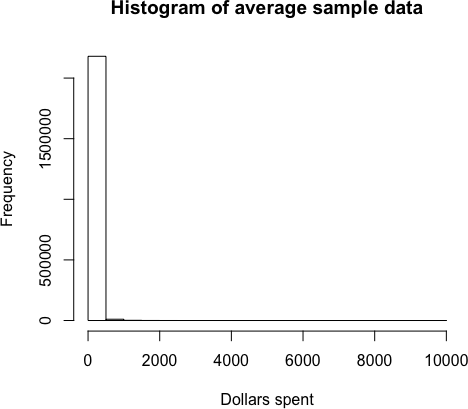
\includegraphics[width=.8 \linewidth]{all-hist.png}
\end{center}
  \vspace{-1em}
  \caption{A histogram of spending amount, generated off of $\frac{1}{348}$ of the \texttt{train} set.}
  \label{fig:spend}
\end{figure}

\begin{figure}[H]
\begin{center}
	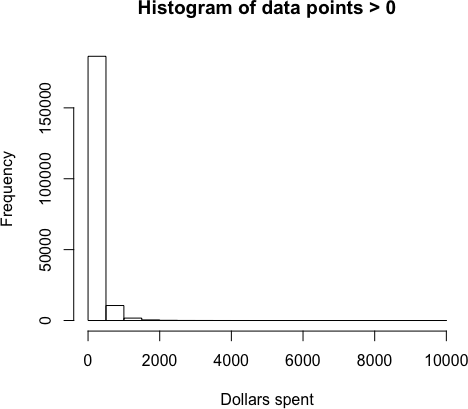
\includegraphics[width=.8 \linewidth]{hist-gt-0.png}
\end{center}
  \vspace{-1em}
  \caption{A histogram of spending amount with non-spenders excluded, generated off of $\frac{1}{348}$ of the \texttt{train} set.}
  \label{fig:spend-non}
\end{figure}

\subsection*{Regression Problem}
We approached regression as merely a way of sorting the output from out classifier, as the second step of our two step process. We would train the regressor on only those households who did spend money, using the household's spending as the label. The first thing we did was to normalize the distribution of spenders through taking the log of the spending amount, as shown in Figures \ref{fig:logspend} and \ref{fig:logspend-non}. Through further experimenting and research, we settled on using slight L1 regularization and a quantile loss function. We used L1 regularization because of how well it deals with sparse feature vectors, and we noticed that it performed significantly better than either L2 regularization or no regularization. A quantile loss function was chosen because it focuses on estimating quantiles (i.e. the top spenders) rather than approximating the median most accurately. Doing this, we were accurate to within $\$2,000$ on average. When testing on those households predicted to spend by our first stage classifier, we were accurate to within $\$1,200$ on average.

\begin{figure}[H]
\begin{center}
	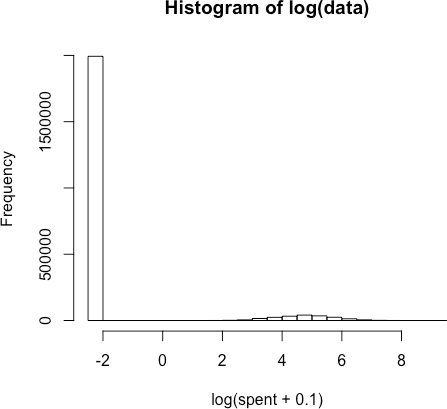
\includegraphics[width=.8 \linewidth]{log-spend.png}
\end{center}
	\vspace{-1em}
	\caption{A histogram of the log of spending amount, generated off of $\frac{1}{348}$ of the \texttt{train} set.}
	\label{fig:logspend}
\end{figure}

\begin{figure}[H]
\begin{center}
	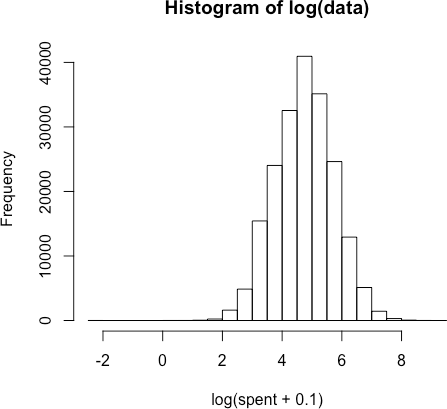
\includegraphics[width=.8 \linewidth]{log-spend-gt-0.png}
\end{center}
	\vspace{-1em}
	\caption{A histogram of the log of spending amount with non-spenders excluded, generated off of $\frac{1}{348}$ of the \texttt{train} set.}
	\label{fig:logspend-non}
\end{figure}

\section*{Analysis}
Overall, our methods did very well. In the final ranking of the competition we were only slightly worse than Oracle themselves, with almost $60\%$ of possible revenue versus the baseline of random guessing at less than $10\%$. 

In retrospect, we should have focused more on tuning the classifier. Analyzing the \texttt{val} dataset, there are only $99,684$ households who spent any money at all, which is less than the $100,000$ we get to put up for advertising. If we could have accurately predicted spender vs non-spender, we would have gotten $100\%$ of revenue. However, other groups in the contest found that there were very few features which had any strong correlation with class label. In fact, out of the $133,531$ features, only around 20 were found to always be strongly associated with one class. The winning group simply spent time tuning the learning rate for their regressor, and found a ``magic value'' which bumped their percent of possible revenue up to $63\%$. 

\section*{Conclusion}
Overall, it seems that this was a really hard problem. We scored only a little less than Oracle's own data scientists, and only 3 percentage points lower than the best result of the competition. This is remarkable for us, as this is our first ``real'' experience with data science and machine learning, and is also our first experience with such large data sets. This has primarily been a learning experience, and has peaked our interest in methods such as distributed computing for dealing with awkwardly large data sets. Additionally, this project did a fantastic job showcasing Vowpal Wabbit. Everything we did with it was bottle necked by disk I/O, which is outstanding for something as complex as linear regression in $133,531$ dimensions. In total, this was a very engaging and difficult project that we were not fully prepared for, but learned a lot from. Scoring decently well is a nice cherry on top of that. 


\section{Appendix: Contest Details}
\label{sec:app1}
\subsection*{Details about the Data}
Each of the three data sets was about 7.8GB compressed, and 35GB fully uncompressed. Additionally, the way we implemented our two step process involved having three copies of the same data, which entailed taking up roughly 300GB of storage all told. Each data set had about 1.2 million households (entries) in it, with each household's feature vector being a sparse vector of size $133,351$. We used a m4.xlarge node from Amazon's EC2 Web Service in order to have a clean workspace, which was perfect for dealing with such a mess of file conversions from the format provided (See \citet{codata_oracle_2016}) to various Vowpal Wabbit formats. 

\subsection*{Details about Scoring}
Scoring had two components: maximum revenue, and maximum number of buyers. Prizes were weighted towards models which achieved a higher maximum revenue, so most every team targeted that. Interestingly, teams which did best at one also did the best at the other. It seems that maximum revenue is most directly linked to predicting spender vs non-spender, rather than predicting spending amount. That is likely due to the fact that there is no benefit from listing the highest spenders first on the list of $100,000$. Listing a high spender as number one has exactly as much benefit as listing them at number nine-thousand. For more information, see \citealt{codata_oracle_2016}.

\section{Appendix: Scripts and Data}
Our code can be found at \citeauthor{cuthbertson_scuthbert/oracleaudiencecompetition_2016}, but the actual data must be obtained through the data science team.  

\newpage
\bibliography{zotero}
\bibliographystyle{icml2015}

\end{document} 